\documentclass{article}
\usepackage{graphicx}
\usepackage[margin=1.5cm]{geometry}
\usepackage{amsmath,amsfonts}

\begin{document}

\title{Tuesday Reading Assessment: Energy and Power in Capacitors}
\author{Prof. Jordan C. Hanson}

\maketitle

\section{Memory Bank}

\begin{itemize}
\item $C_{tot} = C_1+C_2 + ...$ ... Total capacitance for capacitors in parallel.
\item $U = \frac{1}{2} C V^2$ ... Energy stored in a capacitor.
\item $P = U/T$ ... Power consumed in a system, assuming $U$ is energy or work done, and $T$ is time duration.
\end{itemize}

\begin{figure}
\centering
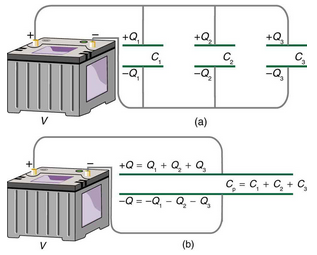
\includegraphics[width=0.4\textwidth]{figures/cap3.png}
\caption{\label{fig:c} A system of three parallel capacitors charged by a battery voltage.}
\end{figure}

\section{Energy and Power with Capacitors}

\begin{enumerate}
\item Suppose a system stores 0.1 J of energy, and releases all of it in 10 ms.  To what power consumption does this correspond? \\ \vspace{1cm}
\item Consider Fig. \ref{fig:c}, in which three parallel capacitors are being charged by a battery voltage.  Suppose we measure the following:
\begin{itemize}
\item $C_1 = 2\mu$F
\item $C_2 = 2\mu$F
\item $C_3 = 4\mu$F
\end{itemize}
(a) What is the total capacitance of the system? (b) If the battery voltage is 12V, how much energy is stored? \\ 
\item If the energy stored in the system in Fig. \ref{fig:c} is released in 10 ms, what is the power provided?
\end{enumerate}

\end{document}
